\documentclass{article}
\usepackage{graphicx} % Required for inserting images

\usepackage{mathtools}
\usepackage{amsmath, amssymb}
\graphicspath{{./images/}}
\usepackage{capt-of}
\usepackage{caption}
\usepackage{subfigure}
\usepackage{subcaption}
\usepackage[utf8]{inputenc}
\usepackage{matlab-prettifier}
\usepackage{authblk}
\usepackage[a4paper,margin=2.5 cm]{geometry}
\usepackage{hyperref} 
\usepackage{enumitem}
\usepackage{upquote}
\usepackage{listings}
\newtheorem{theorem}{Theorem}
\lstset{
    language=Matlab,
    basicstyle=\ttfamily\small,
    breaklines=true,
    keywordstyle=\color{blue},
    stringstyle=\color{purple},
    commentstyle=\color{green!60!black},
    showstringspaces=false,
    literate={"}{{\fontencoding{T1}\selectfont\char34}}1 
}

\title{CMEB Project 1}

\author{Samuele Ferraro}

\date{15 April 2026}

\begin{document}
\maketitle
\newpage
\tableofcontents 
\newpage

\section{Assignment}
   

\begin{enumerate}[label=\alph*)]
    \item \textbf{Flux density in the primal formulation.} Introduce a FEM discretization $J_{h}(x)$ of $J(x)$ by means of piecewise constant polynomials in
    \begin{equation}
        Q_{h}(a,b):=\{v\in L^{2}(a,b):v|_{[x_{i-1},x_{i}]}\in\mathbb{P}_{0}([x_{i-1},x_{i}]) \text{ for } i=1,...,N+1\}
        \label{def:Q_h}
    \end{equation}
    Define a basis for $Q_{h}$ of functions $\{\psi_{i}(x)\}_{i=1}^{N+1}$ defined as

    \begin{equation}
    \psi_{i}(x) =
        \begin{cases}
            1 & \text{if } x \in [x_{i-1}, x_{i}] \\
            0 & \text{otherwise}
        \end{cases}
        \label{BasisFunctionPrimal}
    \end{equation}

    Denote with $\{J_{i}\}_{i=1}^{N+1}$ the degrees of freedom of $J_{h}(x)$.\\
    Integrate the constitutive equation of 
    \begin{equation}
        \begin{cases}
            J'(x) + \sigma u(x) = f(x) & x \in (a, b) \\
            J(x) = -\mu(x) u'(x)  & x \in (a, b) \\
            u(a) = u(b) = 0
        \end{cases}
        \label{PrimalWeakFormulation}
    \end{equation}
    by testing against the basis functions $\psi_{i}(x)$ for $i=1,...,N+1$ and using in place of $u(x)$ and $J(x)$ the corresponding discrete approximations $u_{h}(x)$ and $J_{h}(x)$. By substituting the FEM representations of these two functions, derive an expression for the degrees of freedom of $J_{h}(x)$.

    \item \textbf{Mixed formulation.} We derive and solve for $(u(x),J(x))$ the weak formulation of a slight modification of \eqref{PrimalWeakFormulation}:
    \begin{equation} \label{eq:mixed_strong}
        \begin{cases}
            J'(x) + \sigma u(x) = f(x) & x \in (a, b) \\
            \frac{J(x)}{\mu(x)} + u'(x) = 0 & x \in (a, b) \\
            u(a) = u(b) = 0
        \end{cases}
    \end{equation}
    which intrinsically ensures the mass conservation as $J(x)$ is computed in such a way to satisfy the conservation equation. 
    
    Derive the weak formulation of \eqref{PrimalWeakFormulation} by looking for the solution $(u(x),J(x))\in V\times Q$ with $Q=L^{2}(a,b)$ and testing the conservation equation with functions $v(x)\in V$ and the constitutive law with functions $q(x)\in Q$.
    
    Discretize the weak formulation by looking for $(u_{h}(x),J_{h}(x))\in V_{h}\times Q_{h}$ and testing the weak formulation against functions $(v_{h}(x), q_{h}(x))\in V_{h}\times Q_{h}$. Assemble analytically the linear system arising from the FEM discretization.

    \begin{equation} \label{eq:mixed_system}
        \begin{bmatrix}
            A_{00} & A_{01} \\
            A_{10} & A_{11}
        \end{bmatrix}
        \begin{bmatrix}
            u \\
            J
        \end{bmatrix}
        =
        \begin{bmatrix}
            f_0 \\
            f_1
        \end{bmatrix}
    \end{equation}
    
    where $A_{00} \in \mathbb{R}^{N \times N}$, $A_{01} \in \mathbb{R}^{N \times (N+1)}$, and $f_0 \in \mathbb{R}^N$ are derived from the conservation equation, while $A_{10} \in \mathbb{R}^{(N+1) \times N}$, $A_{11} \in \mathbb{R}^{(N+1) \times (N+1)}$, and $f_1 \in \mathbb{R}^{N+1}$ are derived from the constitutive law.
    
    Compute analitically the degrees of freedom $\{J_{i}\}_{i=1}^{N+1}$ and compare them with those obtained in point a, using the definition $\overline{\overline{\mu}}|_{i}:=(\overline{\mu^{-1}}|_{i})^{-1}$ of the harmonic average of $\mu(x)$ over $[x_{i-1},x_{i}]$. Recall that for $g \in L^1(x_{i-1}, x_i)$ the integral average of a function is defined as:
    \begin{equation} 
        \overline{g}|_i = \frac{1}{h} \int_{x_{i-1}}^{x_i} g(x) \, dx
        \label{AvgFunction}
    \end{equation}
 
    \item \textbf{Implementation.} Implement a Matlab function to solve the diffusion-reaction problem in mixed formulation \eqref{eq:mixed_strong} with signature: \newline
    \begin{center}
        \texttt{function [x, u, J] = gfem\_mixed\_dir\_hom(a, b, N, f, mu, sigma)}, \newline     
    \end{center}
    where \texttt{(a,b)} is the domain, \texttt{N+1} is the number of mesh elements, \texttt{f} and \texttt{mu} are the variable right hand side and diffusion coefficient and \texttt{sigma} is the constant reaction coefficient, \texttt{x} are the mesh nodes, \texttt{u} is the FEM density and \texttt{J} the FEM flux density.

    \item \textbf{Comparison between primal and primal mixed formulations.} Let $a=0$, $b=1$, $\sigma=5$, $\mu(x)=1.5+\sin(30\pi x)$ and $u(x)=x^{5/2}(1-x)$[cite: 83]. The right hand side $f(x)$ can be computed as $f(x)=-\mu^{\prime}(x)u^{\prime}(x)-\mu(x)u^{\prime\prime}(x)+\sigma u(x)$.
    \newline Solve numerically the diffusion-reaction problem in mixed formulation \eqref{eq:mixed_strong} with $N+1=30$ mesh elements and compare the FEM density and flux density with those obtained by solving numerically \eqref{eq:primalFormulation} Comment on the $H^{1}(a,b)$ error on the true density $u(x)$ and on the $L^{2}(a,b)$ error on the true flux density $J(x)$.

    \item \textbf{Convergence analysis.} The following theorem for the convergence of the FEM in mixed formulation holds.

        \begin{theorem}
        Assume that the solution pair of the diffusion-reaction problem \eqref{eq:mixed_strong} 
        is such that $u \in H^2(a,b) \cap H^1_0(a,b)$ and $J \in H^1(a,b)$, and let $h$ be 
        sufficiently small. Then, there exists a constant $C > 0$ independent of $h$ such that
        \begin{equation} \label{eq:convergence_theorem}
            \|u - u_h\|_V + \|J - J_h\|_Q \leq C h \left( \|u\|_{H^2(a,b)} + \|J\|_{H^1(a,b)} \right).
        \end{equation}
        \end{theorem}
        
        Verify numerically the above theorem by computing the left hand side of the inequality 
        \eqref{eq:convergence_theorem} for $N = 3^5, 3^6, 3^7, 3^8, 3^9, 3^{10}$ and the same 
        problem of point d). Plot the error decay and estimate the convergence order analytically. 
        Comment the results in light of the theory.
        \end{enumerate}

\newpage

\section{Point a) development}
Let us define the primal formulation of the problem:
\begin{equation}
    \begin{cases}
        &-(\mu(x)u'(x))' + \sigma u(x) = f(x)\\
        &u(a) = u(b) = 0
    \end{cases}
    \label{eq:primalFormulation}
\end{equation}

The flux $J(x)$ can be defined by using the constitutive law:

\begin{equation*}
    J(x) = - \mu(x) u'(x)
\end{equation*}
The discretization of the flux can be written as:

\begin{equation}
    J_h(x)=\sum_{k=1}^{N+1} J_k \psi_k(x)
    \label{eq:J_hDef}
\end{equation}

To find the discrete flux density $J_h(x) \in Q_h(a,b)$, I expand the equation using the weak formulation and testing it using the basis functions defined in \eqref{BasisFunctionPrimal}. \\
\begin{equation}
    \int_{a}^{b} J_h(x) \psi(x) \, dx = -\int_{a}^{b} \mu(x)u_h'(x) \psi(x) \, dx
    \label{WeakFormA}
\end{equation}
First of all, let us compute the left hand side (LHS) of the equation:
\begin{equation*}
    \int_{a}^{b} J_h(x) \psi(x) \, dx = \int_{x_{i-1}}^{x_i} J_h(x) \, dx =\int_{x_{i-1}}^{x_i} \sum_{k=1}^{N+1} J_k \psi_k(x) \, dx = \sum_{k=1}^{N+1} J_k \int_{x_{i-1}}^{x_i} \psi_k(x) \, dx
\end{equation*}
But
\begin{equation*}
    \begin{cases}
         \int_{x_{i-1}}^{x_i} \psi_k(x) = h &\text{  for } k=i \\
         \int_{x_{i-1}}^{x_i} \psi_k(x) = 0 &\text{  for } k \neq i
    \end{cases}
\end{equation*}
thus the LHS can be written as:
\begin{equation*}
    \int_{a}^{b} J_h(x) \psi(x) \, dx = J_i \cdot h 
\end{equation*}\newline

$u_h$ is defined as:
\begin{equation}
    u_h = \sum_{k=1}^{N} u_k \phi_k(x)
    \label{eq:u_hDef}
\end{equation}
where $\phi_k(x) \in X_h^1(a,b)$ is the globally continuous, piecewise linear basis function (often referred to as the "hat function").

The right hand side (RHS) can be written as:
\begin{align*}
    & -\int_{a}^{b} \mu(x)u_h'(x) \psi(x) \, dx = -\int_{x_{i-1}}^{x_i} \mu(x)u_h'(x) \, dx =  -\int_{x_{i-1}}^{x_i} \mu(x) \left(\sum_{k=1}^{N} u_k \phi_k(x)\right)' \, dx = \\
    &  - \int_{x_{i-1}}^{x_i} \mu(x) \sum_{k=1}^{N} u_k \phi'_k(x) \, dx
\end{align*}
 But 
\begin{equation*}
\phi'_k(x) =
    \begin{cases}
           -\frac{1}{h} &\text{  for } k=i-1 \\
          
           \frac{1}{h} &\text{  for } k = i  \\
          
           0 &\text{ otherwise }  \\
    \end{cases}
\end{equation*}
 Thus the RHS can be written as: 
 \begin{align*}
    -\int_{x_{i-1}}^{x_i} \mu(x) \left(- u_{i-1} \frac{1}{h} + u_i \frac{1}{h} \right) \, dx = -\int_{x_{i-1}}^{x_i} \mu(x) \left(\frac{u_i - u_{i-1}}{h}  \right) \, dx= -\left(\frac{u_i - u_{i-1}}{h}  \right) \int_{x_{i-1}}^{x_i} \mu(x) \, dx
 \end{align*}

Overall \eqref{WeakFormA}:
\begin{align}
    J_i \cdot h &= - \left(\frac{u_i - u_{i-1}}{h}  \right) \int_{x_{i-1}}^{x_i} \mu(x) \, dx \\
    J_i & = - \left(\frac{u_i - u_{i-1}}{h^2}  \right) \int_{x_{i-1}}^{x_i} \mu(x) \, dx
\end{align}
which is the expression of the degrees of freedom of $J_h$. I may go further by using \eqref{AvgFunction}:
\begin{equation}
    J_i  = - \left(\frac{u_i - u_{i-1}}{h}  \right)  \overline{\mu}|_i
    \label{eq:primflux}
\end{equation}

This result can be written in a matrix form, as it have been done in Laboratory 2:
\begin{equation*}
    J=\overline{\mu}|_i S u
\end{equation*}
where:
\begin{equation*}
    S = \frac{1}{h}
    \begin{bmatrix}
        1 & -1 & \dots & 0 & 0 \\
        0 & 1 & \dots & 0 & 0 \\
        \vdots & \vdots & \ddots & 0 & 0 \\
        0 & 0 & \dots & 1 & -1
    \end{bmatrix}      
\end{equation*}

\section{Point b) development}
Starting from the conservation equation of \eqref{eq:mixed_strong}
\begin{equation}
    J'(x)+\sigma u(x) = f(x) 
    \label{ConstituiveEquation}
\end{equation}
let us derive the weak formulation of the problem, using the test function $v \in V = H_0^1(a,b)$:
\begin{align*} 
    \int_a^b (J'(x) + \sigma u(x)) v(x) \, dx = \int_a^b f(x) v(x) \, dx \\
    \int_a^b J'(x) v(x) \, dx + \int_a^b \sigma u(x) v(x) \, dx = \int_a^b f(x) v(x) \,  dx
\end{align*}
The first term at LHS can be extended with the integration by parts:
\begin{align*}
    \int_a^b J'(x) v(x) \, dx= [J(x)v(x)]_a^b - \int_a^b J(x) v'(x) \, dx \\
    \int_a^b J'(x) v(x)\, dx = [J(b)v(b) - J(a) v(a)] - \int_a^b J(x) v'(x) \, dx
\end{align*}
but $v(a)=v(b)=0$ so,
\begin{equation*}
    \int_a^b J'(x) v(x) \, dx= - \int_a^b J(x) v'(x) \, dx
\end{equation*}
At the very end, the conservation equation \eqref{ConstituiveEquation}:
\begin{equation}
    - \int_a^b J(x) v'(x) \, dx  + \int_a^b \sigma u(x) v(x) \, dx = \int_a^b f(x) v(x) \,  dx
    \label{eq:WFConservationLaw}
\end{equation}
Let us now analyze the constitutive law of \eqref{eq:mixed_strong}:
\begin{equation*}
    \frac{J(x)}{\mu(x)} + u'(x) = 0 
\end{equation*}
and formulate the weak formulation with a test function $q \in Q$
\begin{equation}
    \int_a^b \frac{J_(x)}{\mu(x)} q(x) + \int_a^b u'(x) q(x) = 0 
    \label{eq:WFConstitutiveLaw}
\end{equation}

Now I can apply the F.E.M. at \eqref{eq:WFConservationLaw} and at \eqref{eq:WFConstitutiveLaw} by using $J_h$ as defined in \eqref{eq:J_hDef} and $u_h$ as defined as \eqref{eq:u_hDef}. Also the test function have to be substituted with respective basis ones ($v_h \rightarrow \phi(x)$  and $q_h \rightarrow \psi(x)$). 
Let us start from \eqref{eq:WFConservationLaw}:
\begin{equation*}
    - \int_a^b \sum_{k=1}^{N+1} J_k \psi_k(x) \phi_i'(x) \, dx  + \int_a^b \sigma \sum_{k=1}^{N} u_k \phi_k(x) \phi_i(x) \, dx = \int_a^b f(x) \phi_i(x) \,  dx
\end{equation*}
for $i=1,...,N$.

Working on the first term of the LHS: 
\begin{align*}
    - \sum_{k=1}^{N+1} \int_a^b J_k \psi_k(x) \phi_i'(x) \, dx
\end{align*}

I can derive the terms of $A_{01}$ of the matrix \eqref{eq:mixed_system} as:

\begin{equation*}
    A_{01, ik} = - \int_a^b \psi_k(x) \phi_i'(x) \, dx
\end{equation*}

Since the test function $\phi_i(x)$ has non-zero derivative only on the interval $[x_{i-1}, x_{i+1}]$, the integral can be split as:
\begin{equation*}
    A_{01, ik} = - \int_{x_{i-1}}^{x_{i}} \psi_k(x) \phi_i'(x) \, dx - \int_{x_{i}}^{x_{i+1}} \psi_k(x) \phi_i'(x) \, dx 
\end{equation*}

Because the trial function $\psi_k(x)$ is $1$ exclusively on $[x_{k-1}, x_k]$ and $0$ elsewhere, for a given row $i$ the only non-zero results occur when $k=i$ and $k=i+1$:
\begin{equation*}
    A_{01, ik} = 
    \begin{cases}
         - \left( 1 \cdot \frac{1}{h} \cdot h \right) = -1 & \text{for } k = i \\[1ex]
         - \left( 1 \cdot \left(-\frac{1}{h}\right) \cdot h \right) = +1 & \text{for } k = i + 1 \\[1ex]
         0 & \text{otherwise}
    \end{cases}
\end{equation*}

This leads to the assembly of the global matrix $A_{01} \in \mathbb{R}^{N \times (N+1)}$. It is a bi-diagonal rectangular matrix that takes the following sparse form:
\begin{equation*} \label{eq:matrix_A01}
    A_{01} = 
    \begin{bmatrix}
        -1 &  1 &  0 & \dots &  0 &  0 \\
         0 & -1 &  1 & \dots &  0 &  0 \\
    \vdots & \vdots & \ddots & \ddots & \vdots & \vdots \\
         0 &  0 & \dots & -1 &  1 &  0 \\
         0 &  0 & \dots &  0 & -1 &  1
    \end{bmatrix}
\end{equation*}

Working on the second term of the LHS:
\begin{equation*}
    \int_a^b \sigma \sum_{k=1}^{N} u_k \phi_k(x) \phi_i(x) \, dx
\end{equation*}

I can derive the terms of $A_{00}$ of the matrix \eqref{eq:mixed_system}:
\begin{equation*}
    A_{00,ik} = \int_a^b \sigma \phi_k(x) \phi_i(x) \, dx
\end{equation*}
Since the basis function $\phi_i(x)$ has a non-zero value between $x_{i-1}$ and $x_{i+1}$:
 \begin{equation*}
     A_{00,ik} = \int_{x_{i-1}}^{x_{i+1}} \sigma \phi_k(x) \phi_i(x) \, dx = \sigma \int_{x_{i-1}}^{x_{i}}\phi_k(x) \phi_i(x) \, dx + \sigma \int_{x_{i}}^{x_{i+1 }}\phi_k(x) \phi_i(x) \, dx 
 \end{equation*}
 Overall, using the Archimedes's theorem for the calculation of the area of parabolas:
 \begin{equation*}
     A_{00,ik} =
     \begin{cases}
         \sigma \int_{x_{i-1}}^{x_{i}}\phi_k(x) \phi_i(x) \, dx = \sigma \cdot h\cdot \frac{1}{4} \cdot \frac{2}{3} = \frac{\sigma h}{6}&\text{  for } k = i-1 \\
         \int_{x_{i-1}}^{x_{i+1}} \sigma \phi_k(x) \phi_i(x) \, dx = \frac{\sigma h 2}{3}&\text{  for } k = i-1 \\
         \sigma \int_{x_{i}}^{x_{i+1 }}\phi_k(x) \phi_i(x) \, dx = \sigma \cdot h\cdot \frac{1}{4} \cdot \frac{2}{3} = \frac{\sigma h}{6} &\text{  for } k = i+1 \\
         0 &\text{  otherwise}
     \end{cases}
 \end{equation*}

 This leads to the assembly of the global matrix $A_{00} \in \mathbb{R}^{N \times N}$: 
\begin{equation*} \label{eq:matrix_A00}
    A_{00} = \frac{\sigma h}{6}
    \begin{bmatrix}
        4 & 1 & 0 & \dots & 0 \\
        1 & 4 & 1 & \dots & 0 \\
        0 & 1 & 4 & \ddots & \vdots \\
        \vdots & \ddots & \ddots & \ddots & 1 \\
        0 & \dots & 0 & 1 & 4
    \end{bmatrix}
\end{equation*}

The RHS of \eqref{eq:WFConservationLaw}, which will lead to $f_0$, may be written as:
\begin{equation*}
    f_{0,i} = \int_a^b f(x) \phi_i(x) \,  dx
\end{equation*}
for $i=1,...,N$.

Since the basis function $\phi_i(x)$ has a non-zero value between $x_{i-1}$ and $x_{i+1}$:
\begin{equation*}
    \int_{x_{i-1}}^{x_{i+1}} f(x) \phi_i(x) \,  dx = \int_{x_{i-1}}^{x_{i}} f(x) \phi_i(x) \,  dx + \int_{x_{i}}^{x_{i+1}} f(x) \phi_i(x) \,  dx 
\end{equation*}

I may use the \textit{Numerical Quadrature Formula} to compute the integrals:
\begin{align*}
    f_{0,i} & =  f\left( \frac{x_{i-1} + x_i }{2} \right) \int_{x_{i-1}}^{x_{i}} \phi_i(x) \,  dx  +  f\left( \frac{x_{i} + x_{i+1} }{2} \right) \int_{x_{i}}^{x_{i+1}} \phi_i(x) \,  dx = \\
     & = f\left( \frac{x_{i-1} + x_i }{2} \right) \frac{h}{2}  +  f\left( \frac{x_{i} + x_{i+1} }{2} \right) \frac{h}{2} = \frac{h}{2} \left[f\left( \frac{x_{i-1} + x_i }{2} \right) + f\left( \frac{x_{i} + x_{i+1} }{2} \right) \right]
\end{align*}



Let us move on the constitutive equation of \eqref{eq:mixed_strong} 
\begin{equation}
    \frac{J(x)}{\mu(x)} + u'(x) = 0
    \label{eq:Constitutive}
\end{equation}
and apply the same F.E.M. at its weak formulation \eqref{eq:WFConstitutiveLaw} for $i=1,...,N+1$: 
\begin{align*}
    &\int_a^b \frac{J_h(x)}{\mu(x)} \psi_i(x) \, dx+ \int_a^b u'_h(x) \psi_i(x) \, dx = 0 \\
    & \int_a^b \frac{\sum_{k=1}^{N+1} J_k \psi_k(x)}{\mu(x)} \psi_i(x) \, dx + \int_a^b \left(\sum_{k=1}^{N} u_k \phi_k(x)\right)' \psi_i(x) \, dx = 0
\end{align*}

Analyzing the first term of the LHS of the equation
\begin{equation*}
    \int_a^b \frac{\sum_{k=1}^{N+1} J_k \psi_k(x)}{\mu(x)} \psi_i(x) \, dx
\end{equation*}
I can derive the corresponding terms of the matrix $A_{11}$ of \eqref{eq:mixed_system}:
\begin{equation*}
    A_{11,ik} = \int_a^b \frac{\psi_k(x) \psi_i(x)}{\mu(x)} \, dx
\end{equation*}
Because the basis function $\psi_k(x)$ is $1$ exclusively on $[x_{k-1}, x_k]$ and $0$ elsewhere:
\begin{equation*}
    A_{11,ik} = 
    \begin{cases}
        \int_{x_{i-1}}^{x_i} \frac{1 \cdot 1 }{\mu(x)} = \int_{x_{i-1}}^{x_i} \frac{1}{\mu(x)} &\text{  for } k=i \\
        0 &\text{  otherwise} 
    \end{cases}
\end{equation*}
Now I can apply the harmonic average as defined by the assignment and the integral average as \eqref{AvgFunction} for $A_{11,ii}$
\begin{align}
   A_{11,ii} = \int_{x_{i-1}}^{x_i} \frac{1}{\mu(x)} \, dx = h \cdot \overline{\left(\frac{1}{\mu}\right)}\big|_i = h \cdot \overline{\mu^{-1}}\big|_i = \frac{h}{\bar{\bar{\mu}}\big|_i}
   \label{eq:A_11coefficient}
\end{align}

This leads to the assembly of the global matrix $A_{11} \in \mathbb{R}^{(N+1) \times (N+1)}$. Remarkably, it is a purely diagonal matrix:
\begin{equation*} \label{eq:matrix_A11}
    A_{11} = h
    \begin{bmatrix}
        \frac{1}{\overline{\vphantom{\rule{0pt}{1.2ex}}\smash{\overline{\mu}}}|_1} & 0 & \dots & 0 \\
        0 & \frac{1}{\overline{\vphantom{\rule{0pt}{1.2ex}}\smash{\overline{\mu}}}|_2} & \dots & 0 \\
        \vdots & \vdots & \ddots & \vdots \\
        0 & 0 & \dots & \frac{1}{\overline{\vphantom{\rule{0pt}{1.2ex}}\smash{\overline{\mu}}}|_{N+1}}
    \end{bmatrix}
\end{equation*}

In order to evaluate the integral in \eqref{eq:A_11coefficient}, I utilize the \textit{Trapezoidal Rule} for numerical quadrature:
\begin{align}
    A_{11,ii} = \int_{x_{i-1}}^{x_i} \frac{1}{\mu(x)} \, dx \approx \frac{h}{2} \left[ \frac{1}{\mu(x_{i-1})} + \frac{1}{\mu(x_i)} \right]
    \label{eq:HarmMeanQuad}
\end{align}

Moving toward the second term of the LHS:
\begin{equation*}
    \int_a^b \left(\sum_{k=1}^{N} u_k \phi_k(x)\right)' \psi_i(x) \, dx
\end{equation*}
I can derive the corresponding $A_{10}$ matrix of \eqref{eq:mixed_system}:
\begin{equation*}
    A_{10,ik} = \int_a^b \phi'_k(x) \psi_i(x) \, dx
\end{equation*}
Since the test function $\phi_k(x)$ has a non-zero derivative only on the interval $[x_{k-1}, x_{k+1}]$, and the basis function $\psi_i(x)$ is $1$ exclusively on $[x_{i-1}, x_i]$ and $0$ elsewhere:
\begin{align*}
    &A_{10,ik} = \int_{x_{i-1}}^ {x_{i}} \phi'_k(x) \psi_i(x) \, dx  \\
    &A_{10,ik} = 
    \begin{cases}
           \int_{x_{i-1}}^ {x_{i}} \phi'_{i-1}(x) \psi_i(x) \, dx = h \cdot \left( - \frac{1}{h}\right)  \cdot 1 = - 1 &\text{  for } k = i-1 \\
           \int_{x_{i-1}}^ {x_{i}} \phi'_{i}(x) \psi_i(x) \, dx = h \cdot \frac{1}{h}  \cdot 1 =1 &\text{  for } k = i \\
           0 &\text{  Otherwise } 
    \end{cases}
\end{align*}

This leads to the assembly of the global matrix block $A_{10} \in \mathbb{R}^{(N+1) \times N}$:
\begin{equation} \label{eq:matrix_A10}
    A_{10} = 
    \begin{bmatrix}
         1 &  0 &  0 & \dots &  0 \\
        -1 &  1 &  0 & \dots &  0 \\
         0 & -1 &  1 & \dots &  0 \\
    \vdots & \vdots & \ddots & \ddots & \vdots \\
         0 &  0 & \dots & -1 &  1 \\
         0 &  0 & \dots &  0 & -1
    \end{bmatrix}
\end{equation}

The $f_1$ of \eqref{eq:mixed_system} is a vector of zeros because the RHS of \eqref{eq:Constitutive} is nil.
\newline

Overall, the global system can be written has:
\begin{equation*}
    \begin{bmatrix}
        A_{00} & A_{01} \\
        A_{10} & A_{11}
    \end{bmatrix}
    \begin{bmatrix}
        u \\
        J
    \end{bmatrix}
    =
    \begin{bmatrix}
        f_0 \\
        f_1
    \end{bmatrix}
\end{equation*}

The global matrices and vectors, assembled analytically in the previous sections, are defined as follows:

\begin{itemize}
    \item \textbf{Matrix $A_{00} \in \mathbb{R}^{N \times N}$}: 
    \begin{equation*}
        A_{00} = \frac{\sigma h}{6} \text{tridiag}(1, 4, 1)
    \end{equation*}
    
    \item \textbf{Matrix $A_{01} \in \mathbb{R}^{N \times (N+1)}$}: The discrete divergence operator coupling flux to density.
    \begin{equation*}
        A_{01} = 
        \begin{bmatrix}
            -1 &  1 &  0 & \dots &  0 &  0 \\
             0 & -1 &  1 & \dots &  0 &  0 \\
        \vdots & \vdots & \ddots & \ddots & \vdots & \vdots \\
             0 &  0 & \dots & -1 &  1 &  0 \\
             0 &  0 & \dots &  0 & -1 &  1
        \end{bmatrix}
    \end{equation*}

    \item \textbf{Matrix $A_{10} \in \mathbb{R}^{(N+1) \times N}$}:
    \begin{equation*}
        A_{10} = 
        \begin{bmatrix}
             1 &  0 &  0 & \dots &  0 \\
            -1 &  1 &  0 & \dots &  0 \\
             0 & -1 &  1 & \dots &  0 \\
        \vdots & \vdots & \ddots & \ddots & \vdots \\
             0 &  0 & \dots & -1 &  1 \\
             0 &  0 & \dots &  0 & -1
        \end{bmatrix}
    \end{equation*}

    \item \textbf{Matrix $A_{11} \in \mathbb{R}^{(N+1) \times (N+1)}$}:
    \begin{equation*}
        A_{11} = h \cdot \text{diag}\left( \frac{1}{\overline{\vphantom{\rule{0pt}{1.2ex}}\smash{\overline{\mu}}}|_1}, \frac{1}{\overline{\vphantom{\rule{0pt}{1.2ex}}\smash{\overline{\mu}}}|_2}, \dots, \frac{1}{\overline{\vphantom{\rule{0pt}{1.2ex}}\smash{\overline{\mu}}}|_{N+1}} \right)
    \end{equation*}

    \item \textbf{Load Vectors $f_0 \in \mathbb{R}^N$ and $f_1 \in \mathbb{R}^{N+1}$}: 
    \begin{equation*}
        f_{0,i} = \frac{h}{2} \left[ f\left( \frac{x_{i-1} + x_i }{2} \right) + f\left( \frac{x_{i} + x_{i+1} }{2} \right) \right] , \quad \quad f_1 = \mathbf{0}
    \end{equation*}
\end{itemize}


\section{Point c) development}
The code implementing the function \texttt{function [x, u, J] = gfem\_mixed\_dir\_hom(a, b, N, f, mu, sigma)} has been reported in \S \ref{code:mix_gfem}.

\section{Point d) development}
The task has been completed by using the codes reported in  \S \ref{code:mix_gfem}, \S \ref{code:prim_gfem} and \S \ref{code:mainProblem}.
Code \S \ref{code:prim_gfem} was adapted Laboratory 2 by adding the computation of J derived in point a).

The plots of $u$ and $J$ with the data given by point d) assignment are represented in the Figure \ref{fig:u_point_d} and Figure \ref{fig:J_point_d}:
\begin{figure}[h]
    \centering
    \includegraphics[width=0.9\linewidth]{images/u_pointD.eps}
    \caption{$u$ plot with primal and mixed formulation}
    \label{fig:u_point_d}
\end{figure}

\begin{figure}[h]
    \centering
    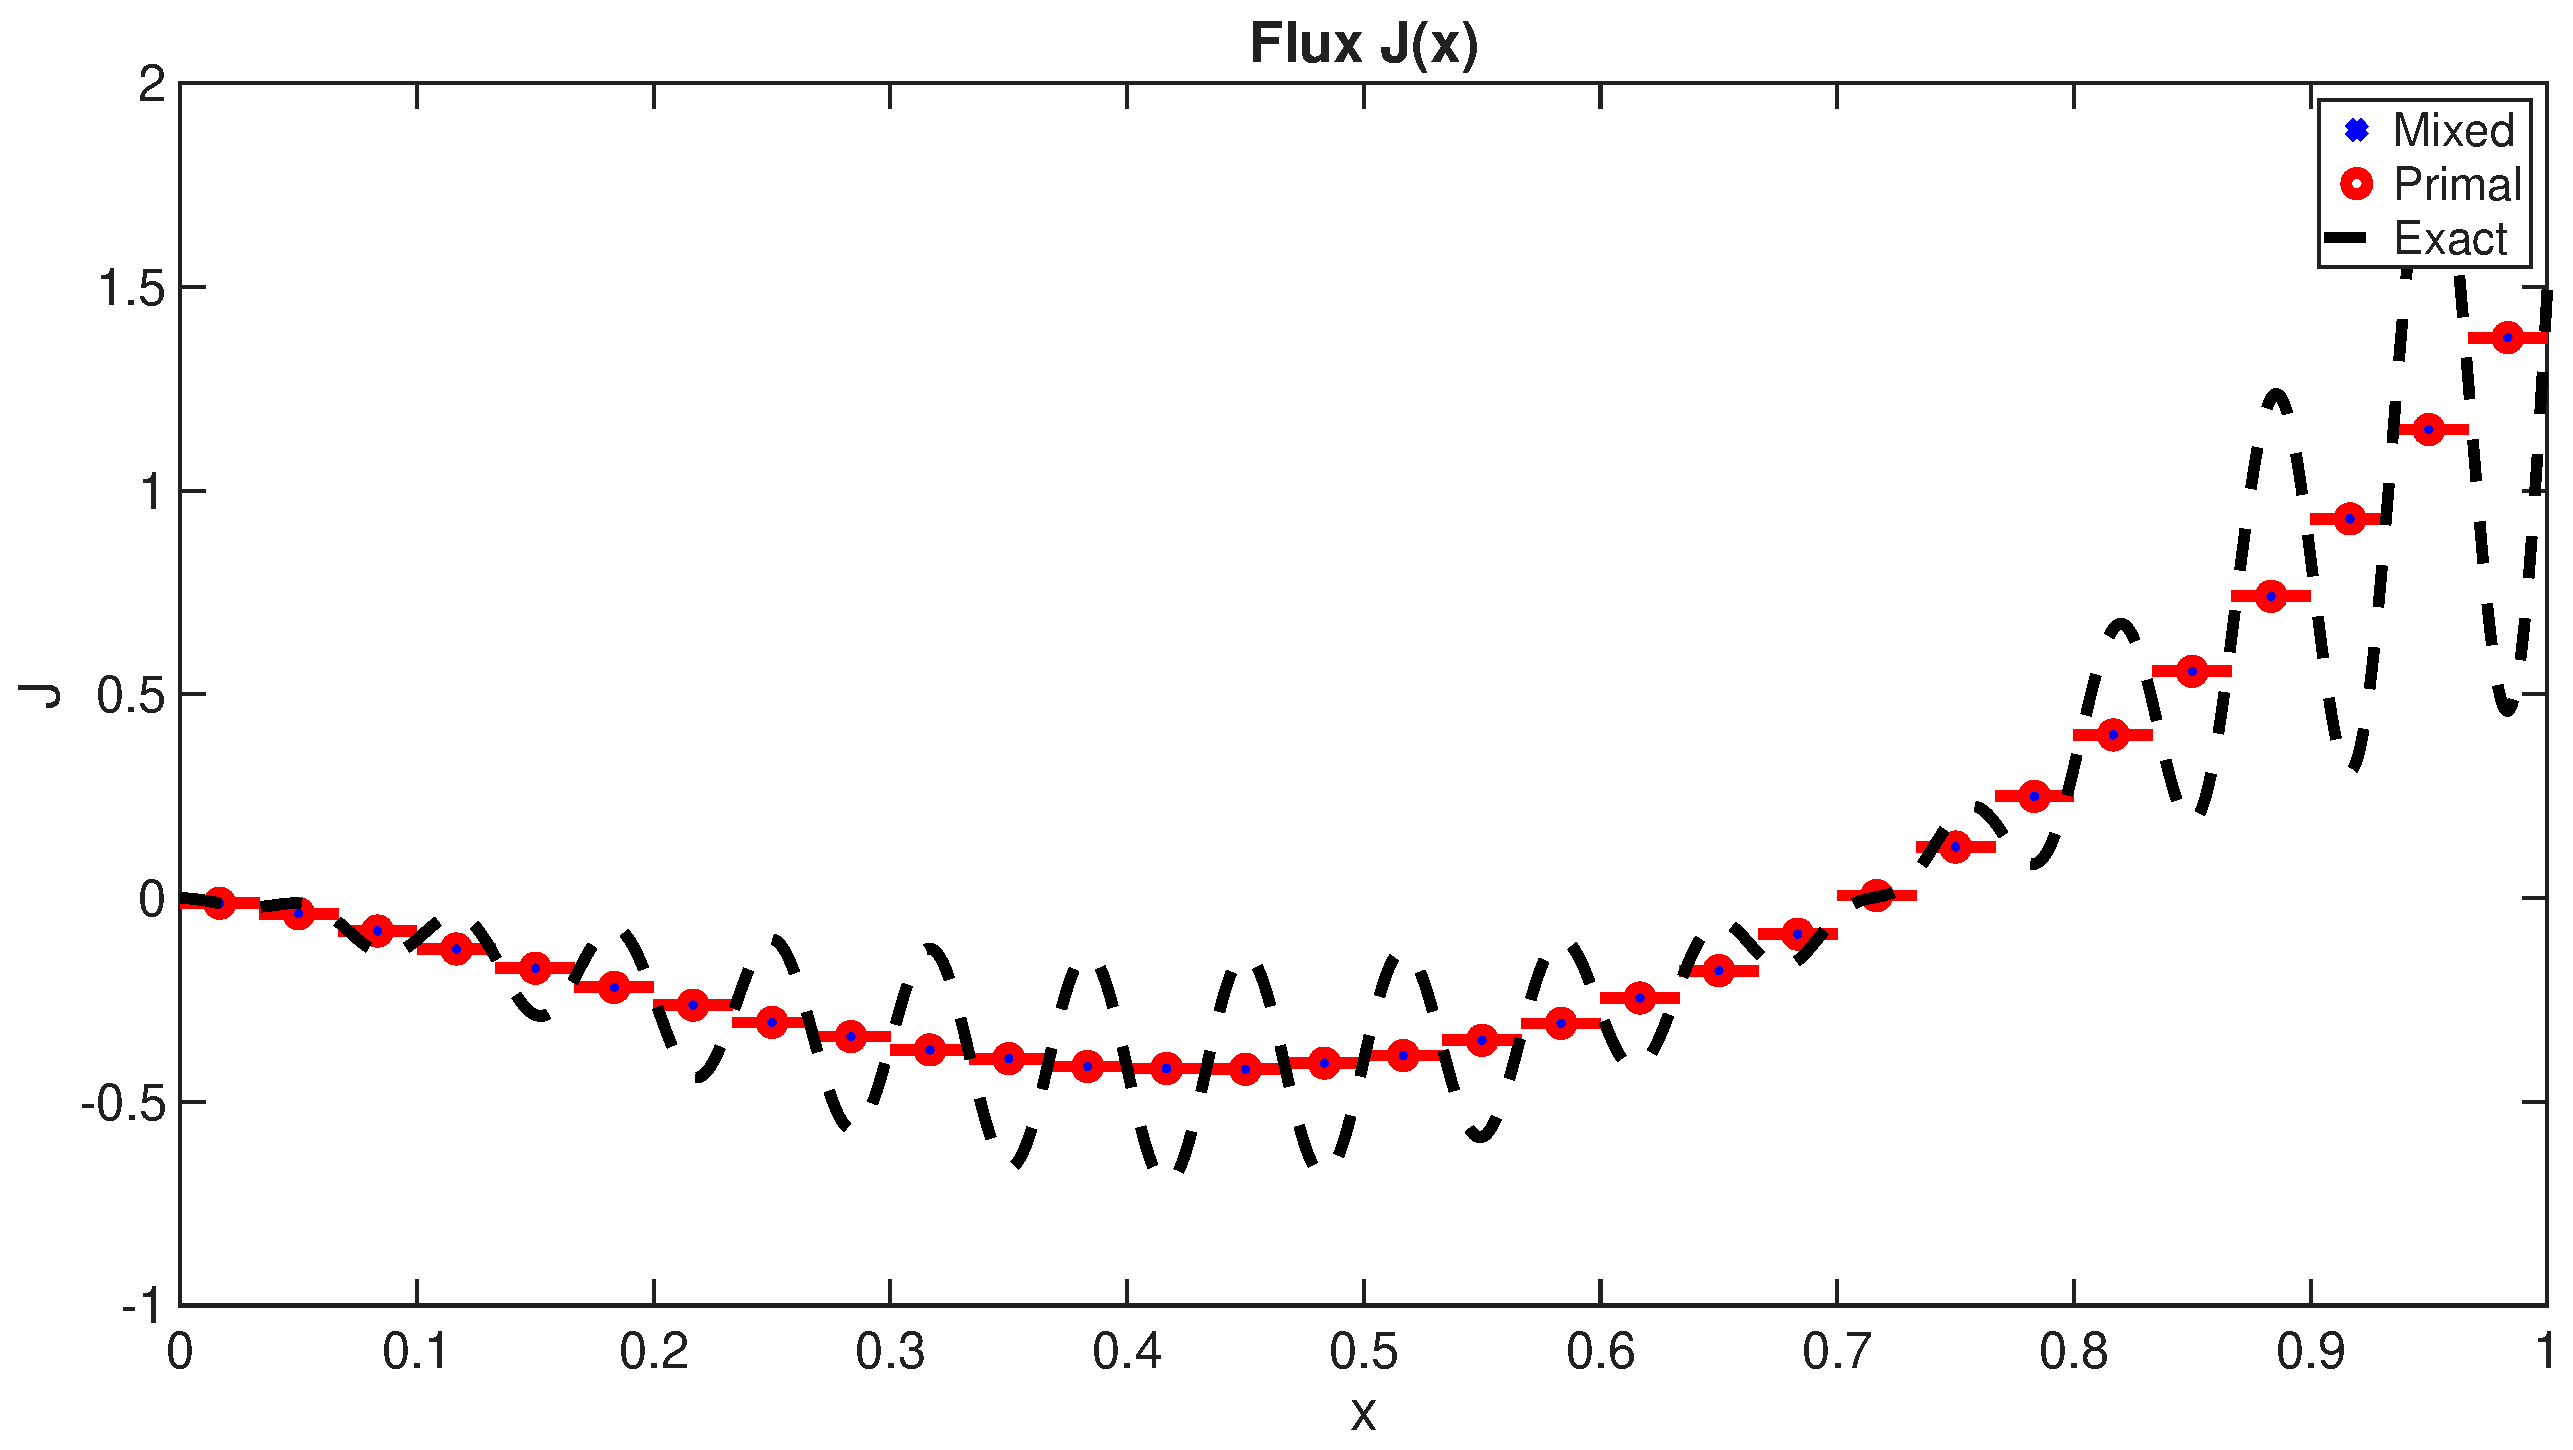
\includegraphics[width=0.9\linewidth]{images/J_pointD.eps}
    \caption{$J$ plot with primal and mixed formulation}
    \label{fig:J_point_d}
\end{figure}

\newpage

While the errors can be seen in Table \ref{tab:errors_d}:
\begin{table}[h]
    \centering
    \begin{tabular}{lcc}
        \hline
        \textbf{Error} & \textbf{Mixed} & \textbf{Primal} \\
        \hline
        $\|u - u_h\|_{H^1(a,b)}$       & $1.9985 \times 10^{-2}$ & $1.9985 \times 10^{-2}$ \\
        $|u - u_h|_{H^1(a,b)}$         & $1.9984 \times 10^{-2}$ & $1.9984 \times 10^{-2}$ \\
        $\|J - J_h\|_{L^2(a,b)}$       & $4.7343 \times 10^{-2}$ & $4.7343 \times 10^{-2}$ \\
        \hline
    \end{tabular}
    \caption{Comparison of errors between mixed and primal formulations 
             with $N+1 = 30$ mesh elements}
    \label{tab:errors_d}
\end{table}

It can be noticed that the two methods lead to the same results and errors.
The reason behind this behavior is the choice of the $N+1$ mesh elements itself: if $N+1 = 30$, the evaluation of the coefficient $\mu_i$ for $i=1,...,N+1$ leads to
\begin{equation}
    \mu_i = 1.5 + sin(30 \pi x_i) = 1.5 + sin\left(30 \pi \frac{i}{N+1}\right) = 1.5 + sin (i \pi) = 1.5  
    \label{eq:sinN29}
\end{equation}
which is a constant value.
If $\mu$ is a constant value then the harmonic mean \eqref{eq:HarmMeanQuad} can be computed as
\begin{equation}
    \frac{1}{\bar{\bar{\mu}}|_i} \approx \frac{1}{2} \left[ \frac{1}{\mu(x_{i-1})} + \frac{1}{\mu(x_i)} \right] = \frac{1}{2} \left[ \frac{1}{1.5} + \frac{1}{1.5}\right] = \frac{1}{1.5}
    \label{eq:HarmMeanQuadConst}
\end{equation}
for every $i = 1,...,N+1$.

While the integral mean, using the same numerical quadrature formula approximation, can be computed as:
\begin{equation}
    \bar{\mu}|_i \approx \frac{1}{2}\left[\mu(x_{i-1}) + \mu(x_i)\right] = \frac{1}{2} (1.5+1.5)=1.5 
    \label{eq:IntegralMeanQuadConst}
\end{equation}
for every $i = 1,...,N+1$.\newline
As demonstrated by equations \eqref{eq:HarmMeanQuadConst} and \eqref{eq:IntegralMeanQuadConst}, the harmonic mean is equal to the integral mean \newline (${\bar{\bar{\mu}}|_i }= \bar{\mu}|_i = 1.5$). \newline
Comparing the primal and the mixed formulation differential equations from \eqref{PrimalWeakFormulation} and \eqref{eq:mixed_strong}:
\begin{align}
    & J(x) = -\mu(x) u'(x)\\
    & \frac{J(x)}{\mu(x)} +u'(x) = 0
\end{align}
it can be easily seen that the main difference between primal and mixed formulation, which is the integration of $\frac{1}{\mu(x)}$ instead of $\mu(x)$, is nullified.  
For the same reason the numerical solutions of $J$ in Figure \ref{fig:J_point_d} does not show any oscillatory behavior, leading to a great discrepancy between numerical and exact solution of J.

\newpage


\section{Point e) development}
This point has been numerically solved by code in \S \ref{code:mainProblem}.
The following Figure \ref{fig:ConvergenceMixed} and Table \ref{tab:convergence_results} show the convergence rate of the problem \eqref{eq:mixed_strong}:

\begin{figure}[h]
    \centering
    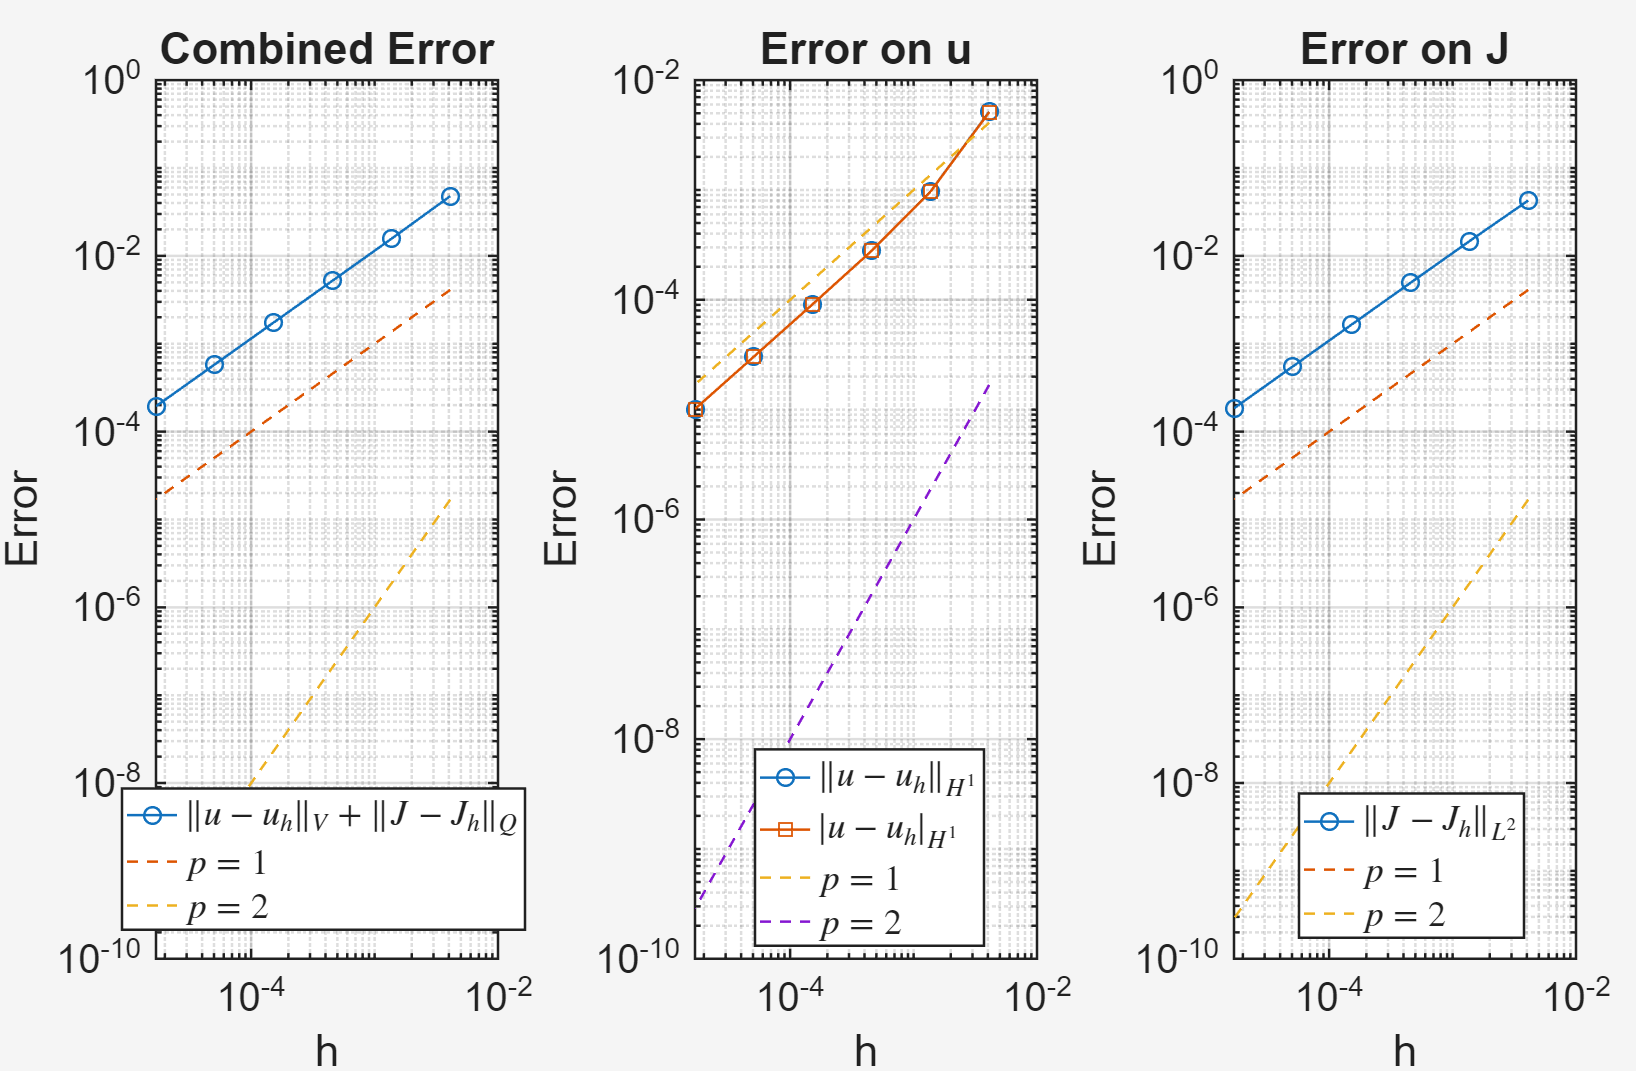
\includegraphics[width=0.9\linewidth]{images/ConvergenceError.png}
    \caption{Convergence rate of the mixed formulation}
    \label{fig:ConvergenceMixed}
\end{figure}

\begin{table}[h]
    \centering
    \renewcommand{\arraystretch}{1.2}
    \begin{tabular}{lccc}
        \hline
        \textbf{Error Type} & \textbf{Norm} & \textbf{Conv. Order ($p$)} & \textbf{Const. ($C$)} \\
        \hline
        Density error       & $\|u - u_h\|_{H^1}$ & $1.0002$ & $0.5998$ \\
        Flux density error  & $\|J - J_h\|_{L^2}$ & $0.9997$ & $10.8443$ \\
        Combined error      & Theorem 1 (LHS)     & $0.9997$ & $11.4441$ \\
        \hline
    \end{tabular}
    \caption{Asymptotic convergence rates and error constants for the mixed formulation.}
    \label{tab:convergence_results}
\end{table}

The convergence rate of the combined error is around 1, as stated by the Theorem \eqref{eq:convergence_theorem}.

Regarding the $u$ error in norm $H^1$ the first order convergence is expected thanks to the proposition 3.6 from the Lecture Notes of part 1:

\textbf{Proposition 3.6} (A priori error estimate in norm V) \textit{if $u \in H^{p+1}(\Omega) \cap V$, for $p \geq 1$, and $u_h \in V_h = V \cap X^r_h (\Omega)$, for $r \geq 1$, then, there exist a constant $C>0$ independent of $h$ and $u \in V$ such that}:
\begin{equation}
    \|u-u_h\|_V \leq C h^s |u|_{H^{s+1}(\Omega)}  \textit{ with } s=min\{r,p\}  \label{prop:u_conv}
\end{equation}
In the case analyzed in this project $r=1$, the convergence order is fixed by $r$ itself.
\newline

Regarding the $J$ error $L^2$, the first order of convergence is still expected due to the proposition 3.7 from the Lecture Notes of part 1:

\textbf{Proposition 3.6} (A priori error estimate in norm $L^2$) \textit{if $u \in H^{p+1}(\Omega) \cap V$, for $p \geq 1$, and $u_h \in V_h = V \cap X^r_h (\Omega)$, for $r \geq 1$, then, there exist a constant $C>0$ independent of $h$ and $u \in V$ such that}:
\begin{equation}
    \|u-u_h\|_{L^2(\Omega)} \leq C h^{s+1} |u|_{H^{s+1}(\Omega)}  \textit{ with } s=min\{r,p\}
    \label{prop:J_conv}
\end{equation}
In the case analyzed in this project, this proposition can be applied by substituting $u$ and $u_h$ with $J$ $J_h$. Considering that the flux $J$ has been discretized with \eqref{def:Q_h}, $r=0$ and the order of convergence is thus $s=1$.
The theorem \eqref{eq:convergence_theorem} is verified because both $\|u - u_h\|_V$  and $\|J - J_h\|_Q $ have an order of convergence equal to one, thus their sum must converge with the same order.

\newpage
For the sake of completeness, Figure \ref{fig:ConvergencePrimal} reports the converge rate of the primal formulation:
\begin{figure}[h]
    \centering
    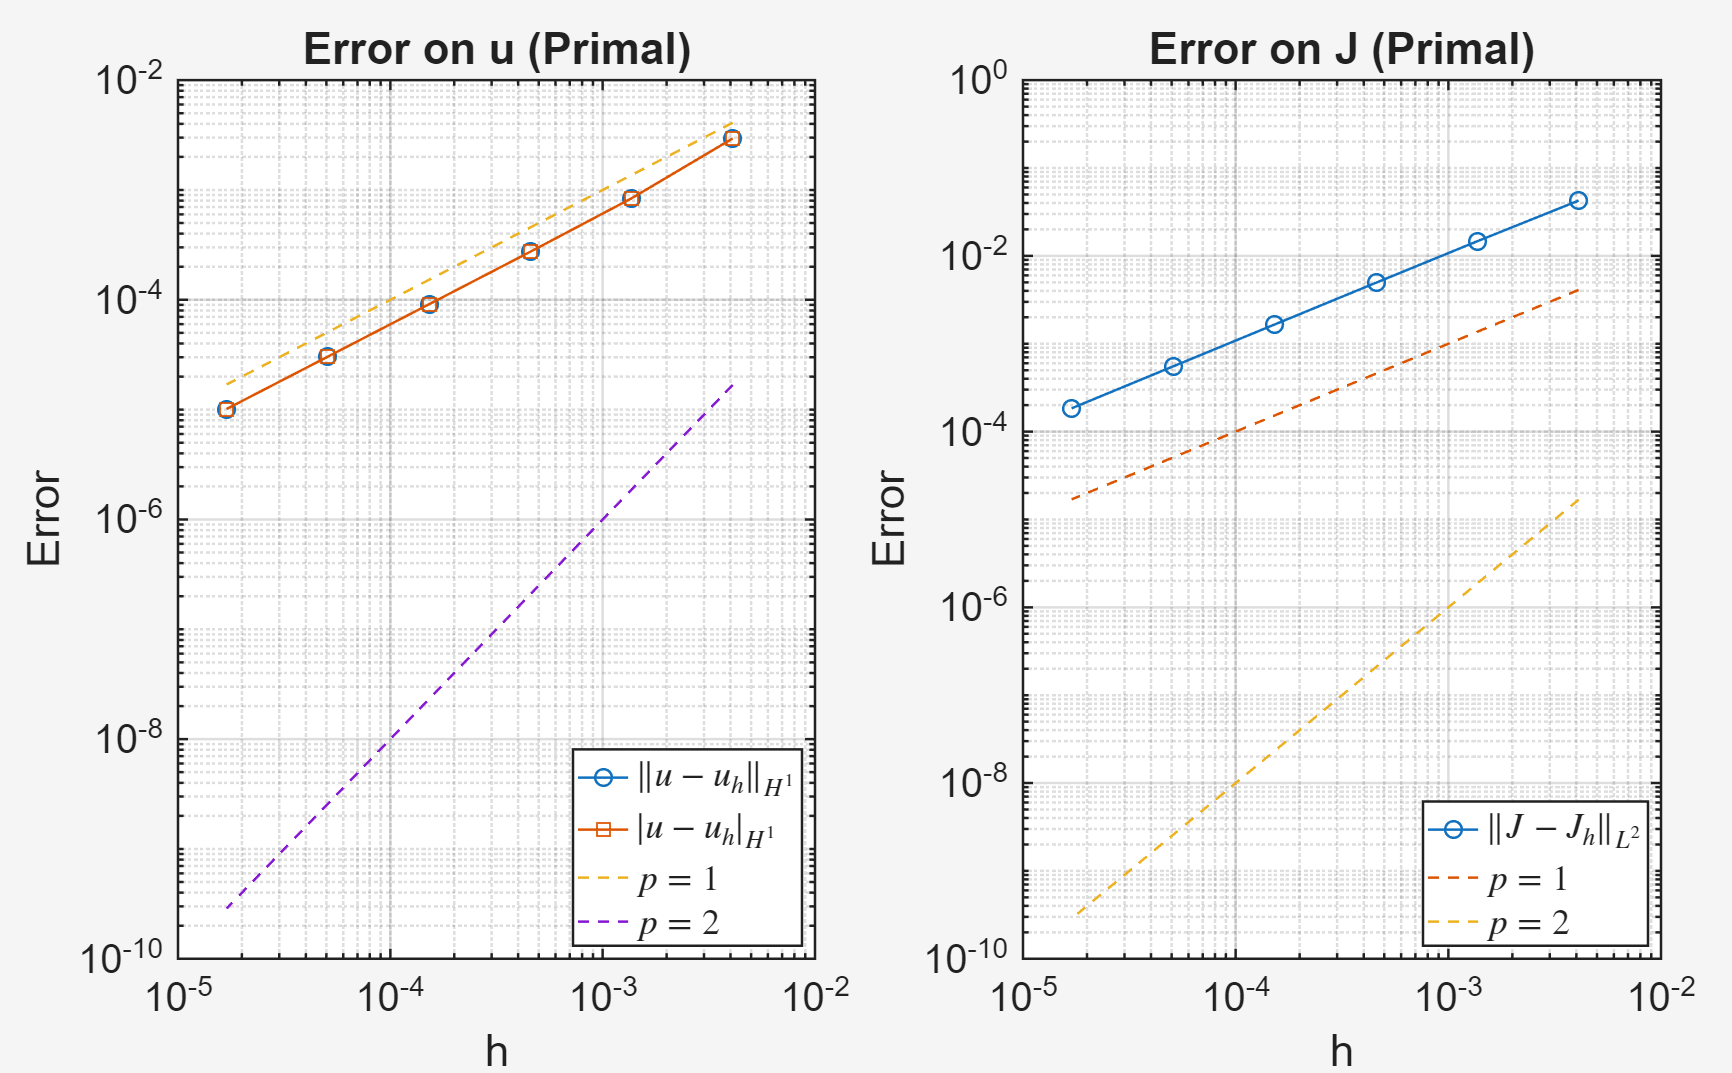
\includegraphics[width=0.9\linewidth]{images/ConvergenceRatePrimal.png}
    \caption{Convergence rate of the primal formulation}
    \label{fig:ConvergencePrimal}
\end{figure}

Its behavior is the same for the mixed one due to \eqref{prop:u_conv} and \eqref{prop:J_conv}

\newpage


\section{Appendix: codes}
\subsection{gfem\_mixed\_dir\_hom.m}
\label{code:mix_gfem}
\begin{lstlisting}[style=matlab-editor]
    function [x, u, J] = gfem_mixed_dir_hom(a, b, N, f, mu, sigma)
% GFEM_MIXED_DIR_HOM Solves the diffusion-reaction problem in mixed formulation
% with homogeneous Dirichlet boundary conditions.
%
% [x, u, J] = gfem_mixed_dir_hom(a, b, N, f, mu, sigma)
%

%space discretization
h =(b-a)/(N+1);
x = linspace(a, b, N+2)'; % Generate the spatial grid points
%defining mid-point 
xm = 0.5 *(x(1:end-1) + x(2:end));

u = zeros(N+2, 1); 
J = zeros(N+1, 1); 

%Build the matrix blocks A_{00} 
e_00 = ones(N,1);

A_00 = sigma*h/6 * spdiags([e_00, 4*e_00, e_00], [-1, 0, 1], N,N);

%Build the matrix blocks A_{01}
A_01 = spdiags([-e_00, e_00], [0,1], N, N+1);

%build the matrix block A_{10}
A_10 = spdiags([-e_00, e_00], [-1, 0], N+1, N);


%Build the matrix block A_{11}
%mu_mean = mu(xm);
%mu_harm_mean = 1./mu_mean; 

%computation of the harmonic mean of the indexes 
mu_harm_mean = arrayfun(@(i) (1/h) * integral(@(t) 1./mu(t), x(i), x(i+1)), 1:N+1)';

A_11 = h*spdiags(mu_harm_mean, 0, N+1, N+1);

A_global = [A_00, A_01;
            A_10, A_11];

%we build the f_0 vector:
f0 = h/2 * f(xm(1:end-1)) + h/2 * f(xm(2:end));
%Building f1
f1 = zeros (N+1,1);
%F global
F_global = [f0;
            f1];
%Solving the system
sol = A_global\F_global;

%the first N elements is u (u(0) and u(N+1) are fixed by boundary condition
u(2:end-1) = sol(1:N);

%The last N+1 element are the flux J
J = sol(N+1:end);

return
\end{lstlisting}

\subsection{gfem\_primal\_dir\_hom.m}
\label{code:prim_gfem}
\begin{lstlisting}[style=matlab-editor]
function [x, u, J] = gfem_primal_dir_hom(a, b, N, f, mu, beta, sigma)
% [x, u, J] = gfem_primal_dir(a, b, N, f, mu, beta, sigma)
%
% This script implements GFEM for the linear advection-diffusion-reaction
% boundary problem:
%
% -(mu(x) u'(x))' + mu u'(x) + sigma*u(x) = f(x)    x in (a,b)
% u(a) = 0
% u(b) = 0
% 
% J is computed in post processing as formulated in Point a) of the report

% space discretization
h = (b-a)/(N+1);
x = linspace(a, b, N+2)';
u = zeros(N+2, 1);

% Mean points of x
xm = 0.5*(x(1:end-1)+x(2:end));

% assembly
e = ones(N,1);

%computation of mu mean via trapezoidal quadrature formula
mu_mean = 0.5*(mu(x(1:end-1)) + mu(x(2:end)));

%Main diagonal of the stiffness matrix: calculated at lecture 2 notes
mu_diag = mu_mean(1:end-1) + mu_mean(2:end);

K = 1/h * spdiags([-[mu_mean(2:end-1); 0], mu_diag, -[0; mu_mean(2:end-1)]], [-1, 0, 1], N, N);

B = beta*0.5 * spdiags([-e, e], [-1, 1], N, N);
M = sigma*h/6 * spdiags([e, 4*e, e], [ -1, 0, 1], N, N);

% We can avoid the modification of the system matrices on the boundary nodes 
% as we are applying Dirichlet BCs
A = K + B + M;

% Midpoint quadrature rule again with
%Computation the rhs
F = h/2 * f(xm(1:end-1)) + h/2 * f(xm(2:end));


% Solve linear system
u(2:end-1) = A\F;

%Computation post processing of J primal
J = -mu_mean .* (u(2:end)-u(1:end-1))/h;

return
    
\end{lstlisting}
\subsection{mainProblem.m}
\label{code:mainProblem}
\begin{lstlisting}[style=matlab-editor]

clear variables
close all
clc

addpath("./supportfunctions");

%parameters
a = 0;
b = 1;
sigma = 5;
N =99;

beta=0;

%Functions given by the assignment and the ones needed to build f
mu = @(x) 1.5 + sin(30*pi*x);
dmu = @(x) 30*pi*cos(30*pi*x);

u_ex = @(x) x.^(5/2) .* (1-x);
du_ex = @(x) 2.5*x.^(1.5).*(1-x) - x.^(5/2);
d2u_ex = @(x) 3.75*x.^(0.5).*(1-x) - 5*x.^(1.5);

J_ex    = @(x) -mu(x) .* du_ex(x);

f = @(x) -dmu(x).*du_ex(x) - mu(x).*d2u_ex(x) + sigma*u_ex(x);

%solving the problem using the two different formulations:
[x_prim, u_prim, J_prim] = gfem_primal_dir_hom(a, b, N, f, mu, beta, sigma);
[x_mix, u_mix, J_mix] = gfem_mixed_dir_hom(a, b, N, f,mu , sigma);

xex = linspace(a, b, 1000)';

% --- Plot u(x) ---
setfonts;
figure;
plot(x_mix, u_mix, '-xb', x_prim, u_prim, '-r', xex, u_ex(xex), '--k');
title('Density u(x)');
xlabel('x');
ylabel('u');
legend('Mixed', 'Primal', 'Exact');


% --- Plot J(x) ---
setfonts;
figure;
hold on
for i = 1:length(J_mix)
    plot([x_mix(i) x_mix(i+1)], [J_mix(i) J_mix(i)], "-b", "HandleVisibility","off");
    plot([x_prim(i) x_prim(i+1)], [J_prim(i) J_prim(i)], "-r", "HandleVisibility","off");   
end
xm = 0.5*(x_mix(1:end-1) + x_mix(2:end));
plot(xm, J_mix, 'xb', xm, J_prim, 'or', xex, J_ex(xex), '--k');
title('Flux J(x)');
xlabel('x');
ylabel('J');
legend('Mixed','Primal', 'Exact');

%%Errors
%Calculation of the errors H1 of u
[err_H1_mix, err_semi_H1_mix] = H1_error(x_mix, u_mix, u_ex, du_ex, 1);
[err_H1_prim, err_semi_H1_prim] = H1_error(x_prim, u_prim, u_ex, du_ex, 1);

fprintf('H1 error on u  - Mixed:  %.6e  (seminorm: %.6e)\n', err_H1_mix, err_semi_H1_mix);
fprintf('H1 error on u  - Primal: %.6e  (seminorm: %.6e)\n', err_H1_prim, err_semi_H1_prim);

%Calculation of the errors L2 of J
err_L2_mix = L2_error(xm, J_mix, J_ex, 0);
err_L2_prim = L2_error(xm, J_prim, J_ex, 0);

fprintf('L2 error on J  - Mixed:  %.6e\n', err_L2_mix);
fprintf('L2 error on J  - Primal: %.6e\n', err_L2_prim);

%% Point e) - Convergence analysis

N_vec = [3^5, 3^6, 3^7, 3^8, 3^9, 3^10];
h_vec = ((b-a) ./ (N_vec + 1))';

%Initialization of the Mixed formulation
err_combined_mix = zeros(length(N_vec), 1);
err_H1_u_mix     = zeros(length(N_vec), 1);
err_semi_H1_u_mix = zeros(length(N_vec), 1);
err_L2_J_mix     = zeros(length(N_vec), 1);

%Initialization of the Primal formulation
err_H1_u_prim     = zeros(length(N_vec), 1);
err_semi_H1_u_prim = zeros(length(N_vec), 1);
err_L2_J_prim     = zeros(length(N_vec), 1);

for k = 1:length(N_vec)
    N_k = N_vec(k);

    %Solve mixed formulation
    [x_mix_k, u_mix_k, J_mix_k] = gfem_mixed_dir_hom(a, b, N_k, f, mu, sigma);
    
    % Compute xm for
    xm_mix_k = 0.5*(x_mix_k(1:end-1) + x_mix_k(2:end));

    % Compute xm for J
  
    % H1 error on u (Mixed)
    [err_H1_u_mix(k), err_semi_H1_u_mix(k)] = H1_error(x_mix_k, u_mix_k, u_ex, du_ex, 1);

    % L2 error on J (Mixed)
    err_L2_J_mix(k) = L2_error(xm_mix_k, J_mix_k, J_ex, 0);

    % Combined error (left hand side of theorem)
    err_combined_mix(k) = err_H1_u_mix(k) + err_L2_J_mix(k);
    
    fprintf('\n--- Combined error per iteration ---\n');
    fprintf('N+1 = %6d | h = %.2e | Err_comb = %.6e\n', N_k+1, h_vec(k), err_combined_mix(k));

    % --- Solve primal formulation ---
    [x_prim_k, u_prim_k, J_prim_k] = gfem_primal_dir_hom(a, b, N_k, f, mu, beta, sigma);
    xm_prim_k = 0.5*(x_prim_k(1:end-1) + x_prim_k(2:end));

    % H1 error on u (Primal)
    [err_H1_u_prim(k), err_semi_H1_u_prim(k)] = H1_error(x_prim_k, u_prim_k, u_ex, du_ex, 1);
    % L2 error on J (Primal)
    err_L2_J_prim(k) = L2_error(xm_prim_k, J_prim_k, J_ex, 0);
end

% --- Estimate convergence order (Mixed) ---
[p_H1_u_mix, C_H1_u_mix] = convergence_rate(err_H1_u_mix, h_vec);
[p_L2_J_mix, C_L2_J_mix] = convergence_rate(err_L2_J_mix, h_vec);
[p_combined_mix, C_comb_mix] = convergence_rate(err_combined_mix, h_vec);

% --- Estimate convergence order (Primal) ---
[p_H1_u_prim, C_H1_u_prim] = convergence_rate(err_H1_u_prim, h_vec);
[p_L2_J_prim, C_L2_J_prim] = convergence_rate(err_L2_J_prim, h_vec);

fprintf('\n--- Estimate of convergence order (Mixed) ---\n');
fprintf('H1(u) order:      %.4f. Computed constant C: %.4f \n', p_H1_u_mix(end),C_H1_u_mix(end));
fprintf('L2(J) order:      %.4f. Computed constant C: %.4f \n', p_L2_J_mix(end), C_L2_J_prim(end));
fprintf('Combined order:   %.4f. Computed constant C: %.4f \n', p_combined_mix(end), C_comb_mix(end));

fprintf('\n--- Estimate of convergence order (Primal) ---\n');
fprintf('H1(u) order:      %.4f. Computed constant C: %.4f \n', p_H1_u_prim(end), C_H1_u_prim(end));
fprintf('L2(J) order:      %.4f. Computed constant C: %.4f \n', p_L2_J_prim(end), C_L2_J_prim(end));

%% Plot of the results (Mixed)
setfonts;
figure('Name', 'Convergence Analysis - Mixed Formulation', 'Position', [100, 100, 1600, 500]);

% --- Subplot 1: Combined error (Theorem 1) ---
subplot(1,3,1);
loglog(h_vec, err_combined_mix, 'o-', ...
       h_vec, h_vec, '--', ...
       h_vec, h_vec.^2, '--', ...
        'LineWidth', 1.5);
grid on;
xlabel('h');
ylabel('Error');
legend('$\|u-u_h\|_V + \|J-J_h\|_Q$', '$p = 1$', '$p = 2$',  ...
       'Interpreter', 'latex', 'Location', 'southeast');
title('Combined Error');

% --- Subplot 2: Error on u (H1 Norm e Seminorm) ---
subplot(1,3,2);
loglog(h_vec, err_H1_u_mix, 'o-', ...
       h_vec, err_semi_H1_u_mix, 's-', ...
       h_vec, h_vec, '--', ...
       h_vec, h_vec.^2, '--', ...
        'LineWidth', 1.5);
grid on;
xlabel('h');
ylabel('Error');
legend('$\|u-u_h\|_{H^1}$', '$|u-u_h|_{H^1}$', '$p = 1$', '$p = 2$', ...
       'Interpreter', 'latex', 'Location', 'southeast');
title('Error on u');

% --- Subplot 3: Error on J (L2 Norm) ---
subplot(1,3,3);
loglog(h_vec, err_L2_J_mix, 'o-', ...
       h_vec, h_vec, '--', ...
       h_vec, h_vec.^2, '--', ...
         'LineWidth', 1.5);
grid on;
xlabel('h');
ylabel('Error');
legend('$\|J-J_h\|_{L^2}$', '$p = 1$', '$p = 2$', ...
       'Interpreter', 'latex', 'Location', 'southeast');
title('Error on J');

%% Plot dei risultati - Primal (1x2)
figure('Name', 'Convergence Analysis - Primal Formulation', 'Position', [150, 150, 1100, 500]);

% --- Subplot 1: Errore su u (Primal) ---
subplot(1,2,1);
loglog(h_vec, err_H1_u_prim, 'o-', ...
       h_vec, err_semi_H1_u_prim, 's-', ...
       h_vec, h_vec, '--', ...
       h_vec, h_vec.^2, '--', ...
        'LineWidth', 1.5);
grid on;
xlabel('h');
ylabel('Error');
legend('$\|u-u_h\|_{H^1}$', '$|u-u_h|_{H^1}$', '$p = 1$', '$p = 2$', ...
       'Interpreter', 'latex', 'Location', 'southeast');
title('Error on u (Primal)');

% --- Subplot 2: Errore su J (Primal) ---
subplot(1,2,2);
loglog(h_vec, err_L2_J_prim, 'o-', ...
       h_vec, h_vec, '--', ...
       h_vec, h_vec.^2, '--', ...
         'LineWidth', 1.5);
grid on;
xlabel('h');
ylabel('Error');
legend('$\|J-J_h\|_{L^2}$', '$p = 1$', '$p = 2$', ...
       'Interpreter', 'latex', 'Location', 'southeast');
title('Error on J (Primal)');


rmpath('./supportfunctions');
\end{lstlisting}

\subsection{Support functions}
    \subsubsection{L2\_error.m}
        \begin{lstlisting}[style=matlab-editor]
            function L2_error = L2_error(x, uh, uex, r)
% Authors: A. Tonini
%
% err = L2_error(x, uh, uex, r)
%
% This script evaluates the L2 error between a FEM approximate 
% solution uh (vector of dofs) evaluated at nodes x and the exact 
% solution uex (function handle)
%
% x: nodes vector
% uh: nodal FEM solution
% uex: exact solution function handle
% r: polynomial degree

% Number of elements
Ne = (length(x) - 1)/max(r,1);
L2_error = 0;

% Gauss quadratures on a reference element [-1,1].
% You need to transform the gauss points from the reference
% element to the one on which we are integrating
switch r
    case 0
        gauss_pts  = 0;
        gauss_w    = 2;
        % Basis functions on the reference element [-1,1]
        Nphi = @(x) 1.0+0.0*x;
    case 1
        gauss_pts  = [-1/sqrt(3), 1/sqrt(3)];
        gauss_w    = [1, 1]';
        % Basis functions on the reference element [-1,1]
        Nphi = @(x) [0.5*(1-x); 0.5*(1+x)];
    case 2
        gauss_pts  = [-sqrt(3/5), 0, sqrt(3/5)];
        gauss_w    = [5/9, 8/9, 5/9]';
        % Basis functions on the reference element [-1,1]
        Nphi = @(x) [0.5*x.*(x-1); 1-x.^2; 0.5*x.*(x+1)];
    otherwise
        error("FEM for polynomial degree %d not implemented.\n", r);
end
Nphi_q = Nphi(gauss_pts);

Nq = length(gauss_w);
local_dofs = r+1;
for e = 1:Ne
    if r == 0
        x1 = x(e);
        x2 = x(1+e);

        % Local degrees of freedom
        uh_local = uh(e);
    else
        x1 = x(1+r*(e-1));
        x2 = x(1+r*e);
        
        % Local degrees of freedom
        uh_local = uh(1+r*(e-1):1+r*e);    
    end
    he = x2 - x1;
    
    % Mapping from the reference element [-1,1] to the element
    % [x(1+r*(e-1)), x(1+r*e)]
    xq = 0.5*(x2-x1)*gauss_pts+0.5*(x2+x1);
    
    % Jacobian of the transformation for the integral on the element e
    J  = he/2;
        
    % Cycle over the quadrature nodes
    for q = 1:Nq
        u_q_local = 0;
         % Cycle over the basis functions
        for i = 1:local_dofs
            u_q_local = u_q_local + uh_local(i)*Nphi_q(i,q);
        end
        L2_error = L2_error + J * gauss_w(q) * (u_q_local - uex(xq(q)))^2;
    end
end

L2_error = sqrt(L2_error);

end
        \end{lstlisting}
    \subsubsection{H1\_error.m}
        \begin{lstlisting}[style=matlab-editor]
            function [H1_error, H1_seminorm] = H1_error(x, uh, uex, duex, r)
% Authors: A. Tonini
%
% err = H1_error(x, uh, uex, duex, r)
%
% This script evaluates the H1 error between a FEM approximate 
% solution uh (vector of dofs) evaluated at nodes x and the exact 
% solution uex (function handle)
%
% x: nodes vector
% uh: nodal FEM solution
% uex: exact solution function handle
% duex: exact derivative function handle
% r: polynomial degree

% Number of elements
Ne = (length(x) - 1)/r;
L2_part = 0;
H1_part = 0;

% Gauss quadratures on a reference element [-1,1].
% You need to transform the gauss points from the reference
% element to the one on which we are integrating
switch r
    case 1
        gauss_pts  = [-1/sqrt(3), 1/sqrt(3)];
        gauss_w    = [1, 1]';
        % Basis functions on the reference element [-1,1]
        Nphi = @(x) [0.5*(1-x); 0.5*(1+x)];
        dNphi = @(x) [-0.5+0.*x; 0.5+0.*x];
    case 2
        gauss_pts  = [-sqrt(3/5), 0, sqrt(3/5)];
        gauss_w    = [5/9, 8/9, 5/9]';
        % Basis functions on the reference element [-1,1]
        Nphi = @(x) [0.5*x.*(x-1); 1-x.^2; 0.5*x.*(x+1)];
        dNphi = @(x) [x-0.5; -2*x; x+0.5];
    otherwise
        error("FEM for polynomial degree %d not implemented.\n", r);
end
Nphi_q = Nphi(gauss_pts);
dNphi_q = dNphi(gauss_pts);

Nq = length(gauss_w);
local_dofs = r+1;
for e = 1:Ne
    x1 = x(1+r*(e-1));
    x2 = x(1+r*e);
    he = x2 - x1;
    
    % Local degrees of freedom
    uh_local = uh(1+r*(e-1):1+r*e);
    
    % Mapping from the reference element [-1,1] to the element
    % [x(1+r*(e-1)), x(1+r*e)]
    xq = 0.5*(x2-x1)*gauss_pts+0.5*(x2+x1);
    
    % Jacobian of the transformation for the integral on the element e
    J  = he/2;
        
    % Cycle over the quadrature nodes
    for q = 1:Nq
        u_q_local = 0;
        du_q_local = 0;
         % Cycle over the basis functions
        for i = 1:local_dofs
            u_q_local = u_q_local + uh_local(i)*Nphi_q(i,q);
            du_q_local = du_q_local + 2/he*uh_local(i)*dNphi_q(i,q);
        end
        L2_part = L2_part + J * gauss_w(q) * (u_q_local - uex(xq(q)))^2;
        H1_part = H1_part + J * gauss_w(q) * (du_q_local-duex(xq(q)))^2;
    end
end

H1_error = sqrt(L2_part+H1_part);
H1_seminorm = sqrt(H1_part);

end
        \end{lstlisting}
    \subsubsection{convergence\_rate.m}
        \begin{lstlisting}[style=matlab-editor]
            function [p, C] = convergence_rate(err, h)
% this function estimates the order of convergence p and the asymptotic 
% error constant C of a sequence of errors contained in the vector err
% [p, C] = order_estimate(err)
%
p = log2(err(1:end-1)./err(2:end))./log2(h(1:end-1)./h(2:end));
%
C = err(1:end-1)./(h(1:end-1).^p);
return
        \end{lstlisting}
\end{document}

